		\begin{align}
	\vec{n}=\myvec{\sqrt{3}\\1},
			c=-2
			\\
			\implies
			\theta=\tan^{-1}\brak{\frac{1{{\sqrt{3}}}
			=\frac{\pi}{6},
			p=\frac{\abs{c}}{\norm{\vec{n}}}=1
		\end{align}
		\iffalse
See \figref{fig:chapters/11/10/4/2/Fig1}.
\begin{figure}[H]
	\begin{center} 
	    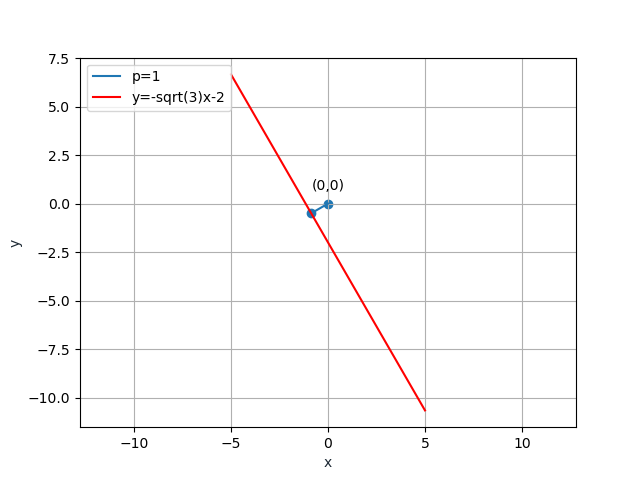
\includegraphics[width=0.75\columnwidth]{chapters/11/10/4/2/figs/line.png}
	\end{center}
\caption{}
\label{fig:chapters/11/10/4/2/Fig1}
\end{figure}
\fi
